\chapter{Stima del modello del sistema}\label{cap:stimaModello}

\begin{minipage}{12cm}\textit{
		In questo capitolo viene affrontato il problema della stima dei parametri del modello reale, in un equivalente lineare matematico, necessario per le simulazioni future e validare i risultati matematici precedenti.}
\end{minipage}

\vspace*{1cm}
\noindent
Partendo dall'esperimento con l'\nameref{lst:ondaTrapezoidale} per eccitare il sistema senza raggiungere la saturazione della tensione $ V_2 $ (ricordiamo che in uscita abbiamo un derivatore filtrato, quindi ogni onda quadra genera automaticamente una forte derivata), si è puntato a ricavare un modello lineare prima della corrente in $ I_T $ e successivamente della tensione $ V_2 $.\\
Essendo il driver di corrente intrinsecamente non lineare, specie nei pressi della Dead-zone, il cui taglio si è visto non essere netto come si spererebbe, si è cercato di ottenere un buon fitting nei transitori del sistema, dove la dinamica è più lineare e "pulita".\\
Questa stima è ovviamente semi-qualitativa (non troppo affidabile) e ha lo scopo di fornire un modello dell'impianto reale da usare in simulazione durante lo sviluppo del sistema di controllo, le \nonLinearita presenti vengono in questo modello ignorate, ma avendo dinamiche molto rapide, il controllo pensato per il modello lineare che stiamo per ricavare vedremo in seguito, continua ad essere valido anche nel caso reale \nonLineare.\\
Il modello stimato è per $ P_{pos} $ (eq \ref{eq:FuncTrasfTotPos}), al fine di renderne la trattazione più semplice evitando di confondersi con i segni.

\newpage

\section{Metodo di stima automatico}
Il metodo di stima automatico è basato sull'uso del \cite*{IdentificationToolbox} di Matlab, ed è usato allo scopo di ottenere una funzione di trasferimento SISO tra l'ingresso del Duty-Cycle (PWM) e la tensione sul secondario $ V_2 $.\\
Avendo a disposizione anche i dati della corrente sul primario, anche se poco sensibili, si è deciso di dividere la stima in 2 fasi per semplificare il lavoro al Toolbox: prima si è stimato il modello della \textbf{Corrente del Trasformatore} ($ I_1 $), e a causa della sua scarsa sensibilità di misura (risultato \ref{result:Istep}) si è usato il segnale ricostruito come ingresso per la stima della dinamica della tensione sul secondario.\\
Il numero di \textit{Poli} e \textit{Zeri} di entrambe le funzioni di trasferimento sono state scelte partendo dall'analisi teorica descritta nella sezione \nameref{subsec:ModelloFisico}, e il codice è presente in appendice a \nameref{lst:autoEst}.

\begin{table}[H]
	\centering
	\caption[Stime parametri con \cite*{IdentificationToolbox}]{Stime parametri con \cite*{IdentificationToolbox}}		\label{tab:stimaAutomaticaParametri}
	\vspace{1mm}
	\begin{tabular}[t]{||l|c|c||}
		\hline
		\multicolumn{1}{||c}{\textbf{Funzione}}            & \multicolumn{1}{|c}{\textbf{Input}} & \multicolumn{1}{|c||}{\textbf{Output}} \\
		\hline\hline
		                                                   &                                     &                                        \\[-3mm]
		$\hat{P}_{p_{wm} I_1}(s) = \frac{970}{s+110}$      & PWM                                 & $I_1$                                  \\[3mm]

		$\hat{P}_{I_1 V_2}(s) = -\frac{0.44\,s+11}{s+200}$ & $I_1$                               & $V_2$                                  \\[3mm]

		$\hat{P}_{p_{wm} V_2}(s) = -\frac{430\,s+11+4}{s^2+310\,s+26}$
		                                                   & PWM                                 & $ V_2 $                                \\
		\hline
	\end{tabular}
\end{table}
\noindent
Il risultato è che la stima del primario ha un aspetto simile a quello che ci aspettavamo, ma il secondario già sbaglia completamente aggiungendo un guadagno fisso nel numeratore che non dovrebbe esistere, e un segno '$ - $' che non ha senso di essere rispetto ai dati usati per l'identificazione.\\
Di seguito la simulazione delle prime 2 funzioni di trasferimento (essendo la 3° la loro moltiplicazione ha poco senso mostrarla in simulazione sugli stessi dati).

\begin{figure}[H]
	\centering
	\caption[Simulazione con stima automatica]{Simulazione con stima automatica}
	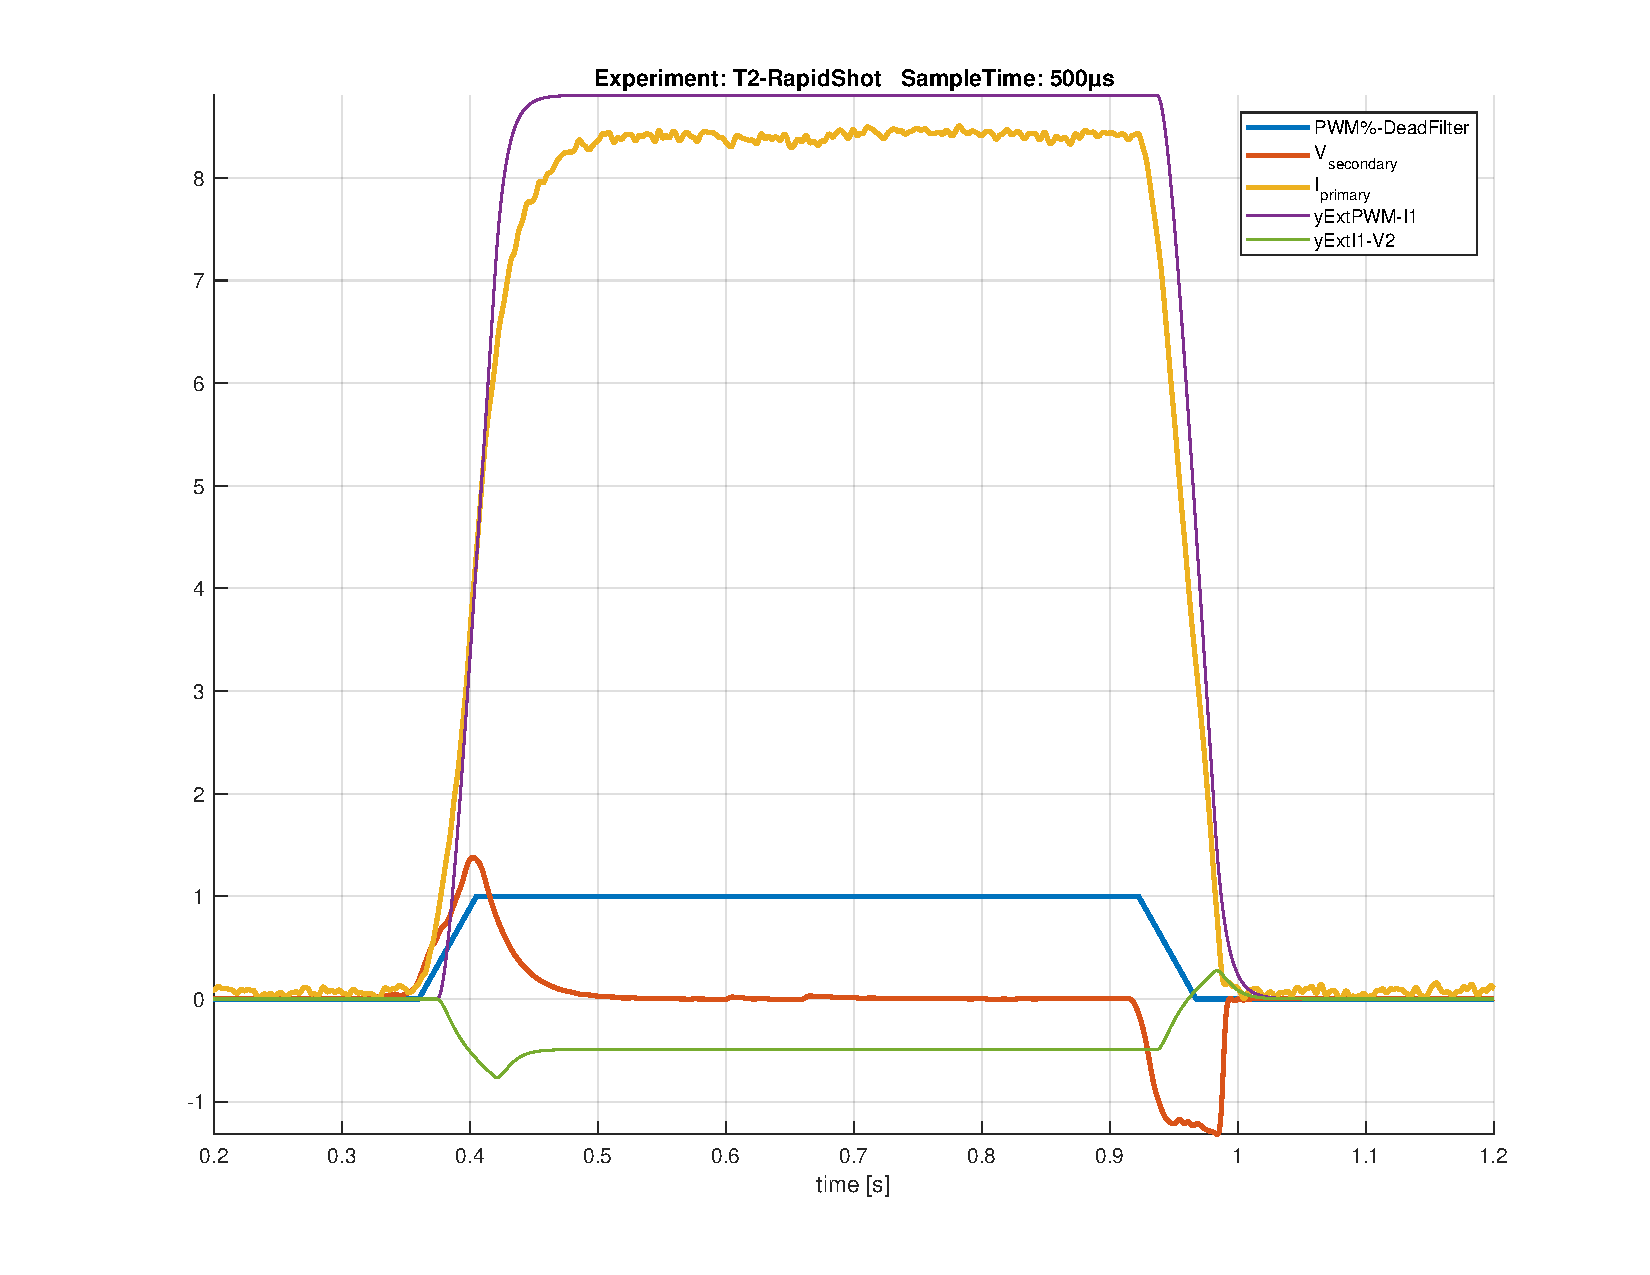
\includegraphics[width=1\textwidth]{Stime/T2-RapidShot-autoExt.pdf}
\end{figure}

\noindent
Analizzando il grafico abbiamo che i primi 3 segnali (spessi), sono i dati reali dell'esperimento filtrati (\nameref{subsec:filtraggio}), mentre le altre 2 linee rappresentano la simulazione usando la stima del Toolbox come modello.\\
Risulta facile vedere che la corrente del primario è accettabile anche se migliorabile, ma la funzione di trasferimento stimata per il secondario è completamente sbagliata, anche se dimensionalmente è simile.\\
Usando queste stime come base si sono trovati a mano dei coefficienti che meglio approssimano l'andamento delle curve.


\section{Tuning dei coefficienti}
Partendo dai modelli generati da \cite*{IdentificationToolbox} e riportati in tabella \ref{tab:stimaAutomaticaParametri}, si sono '\textit{limati}' i dati a mano per migliorare la stima dei parametri, di seguito è riportata la tabella con i valori migliorati:
\begin{table}[H]
	\centering
	\caption[Stime parametri tarati a mano]{Stime parametri tarati a mano}		\label{tab:stimaManualeParametri}
	\vspace{1mm}
	\begin{tabular}[t]{||l|c|c||}
		\hline
		\multicolumn{1}{||c}{\textbf{Funzione}}                                                & \multicolumn{1}{|c}{\textbf{Input}} & \multicolumn{1}{|c||}{\textbf{Input}} \\
		\hline\hline
		                                                                                       &                                     &                                       \\[-3mm]
		$\tilde{P}_{p_{wm} I_1}(s) = \frac{8.4}{0.022\,s+1}$                                   & PWM                                 & $I_1$                                 \\[3mm]

		$\tilde{P}_{I_1 V_2}(s) = \frac{\num{8.5e-3}\,s}{\num{3.6e-4}\,s+1}$                   & $I_1$                               & $V_2$                                 \\[3mm]

		$\tilde{P}_{p_{wm} V_2}(s) = \frac{\num{9.1e+3}\,s}{s^2+\num{2.8e+3}\,s+\num{1.3e+5}}$ & PWM                                 & $ V_2 $                               \\
		\hline
	\end{tabular}
\end{table}

\begin{figure}[H]
	\centering
	\caption[Simulazione con parametri tarati a mano]{Simulazione con parametri tarati a mano}
	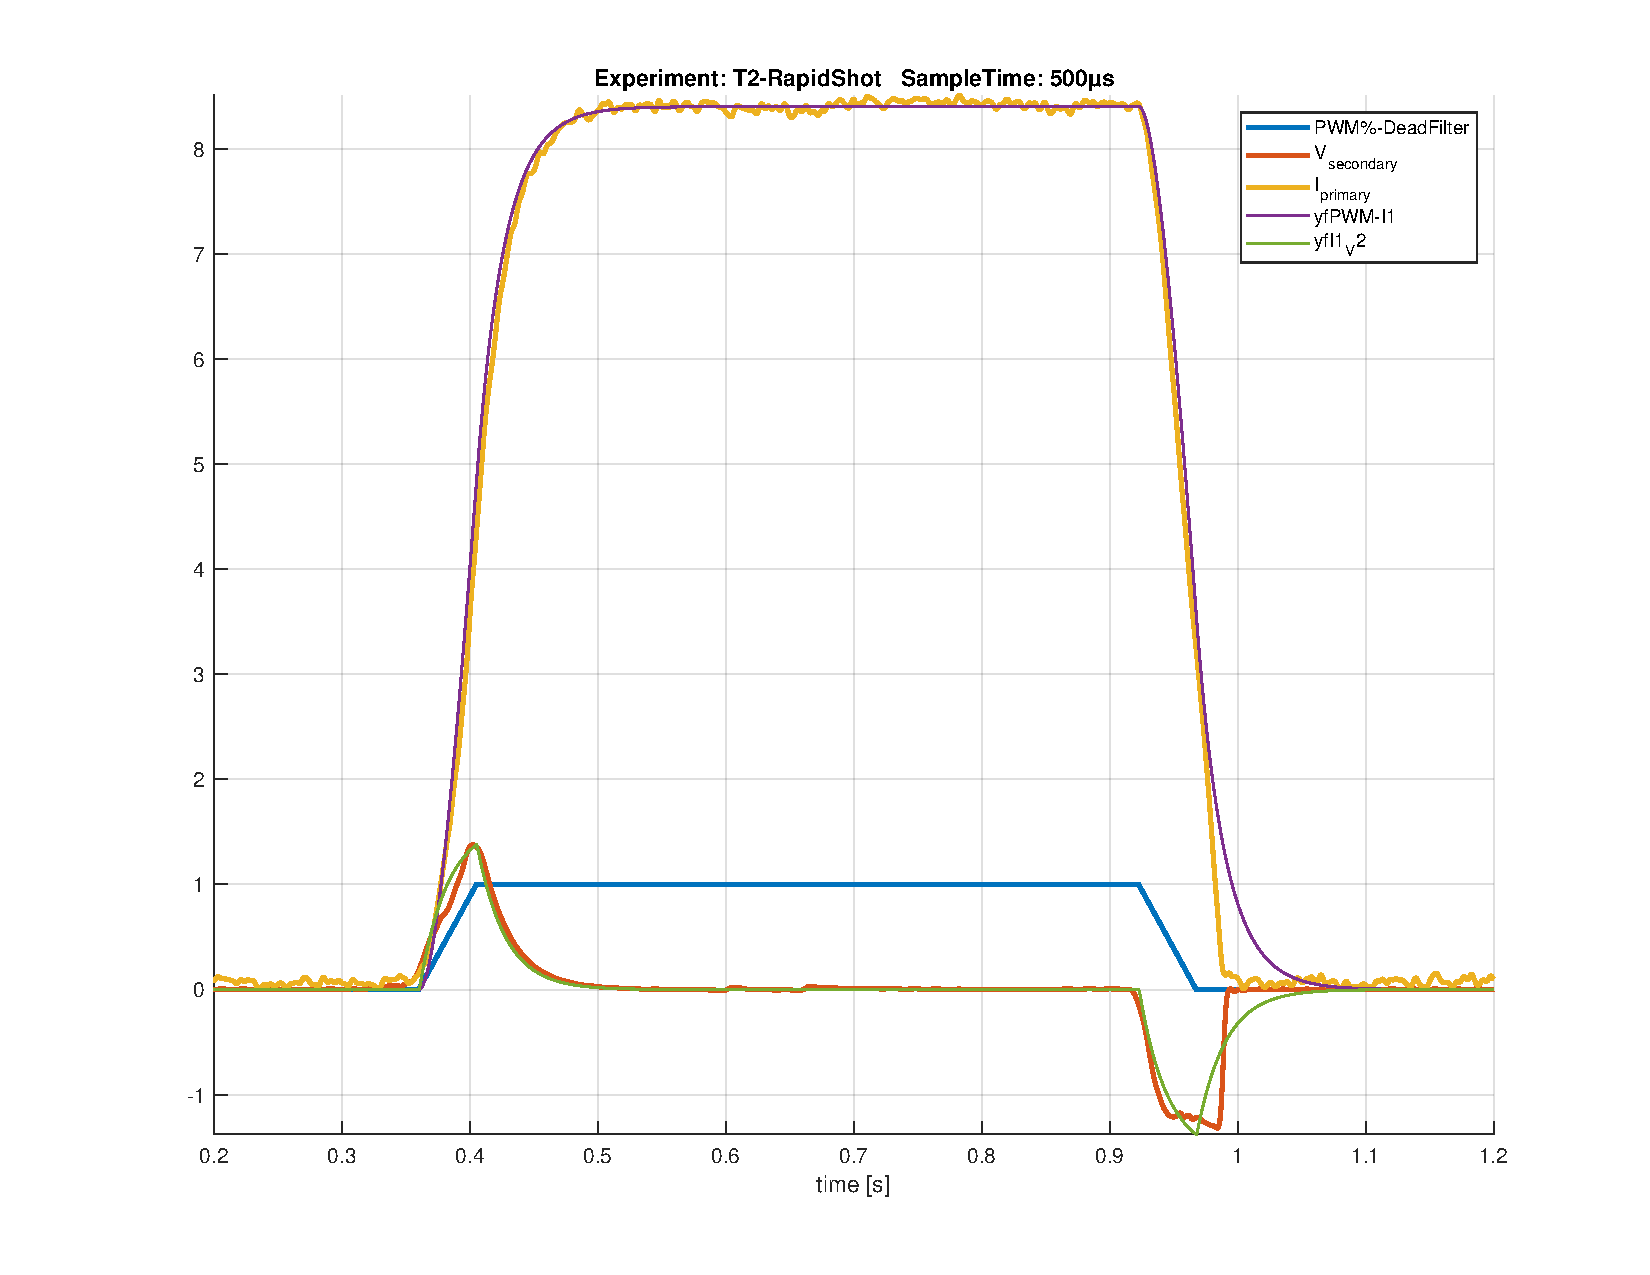
\includegraphics[width=1\textwidth]{Stime/T2-RapidShot-manualExt.pdf}
\end{figure}
\noindent
In particolare nella Dead-Zone inferiore il modello non risulta accurato, essendo predominanti le dinamiche non lineari, e ciò si vede particolarmente bene sul fronte di discesa del sistema, ma nel complesso la funzione trovata è una buona candidata per uno studio teorico e simulativo del sistema prima di passare alla fase implementativa reale.

\section{Benchmark della stima}
In questa sezione andiamo testare la qualità della stima ottenuta dando in ingresso al modello lo stesso input di un segnale eterogeneo con varie forme d'onda.\\
Metteremo quindi a confronto l'andamento reale con quello simulato preso in alcune frazioni interessanti.
\begin{figure}[H]
	\centering
	\caption[Esperimento di verifica della stima 1]{Esperimento di verifica della stima 1}
	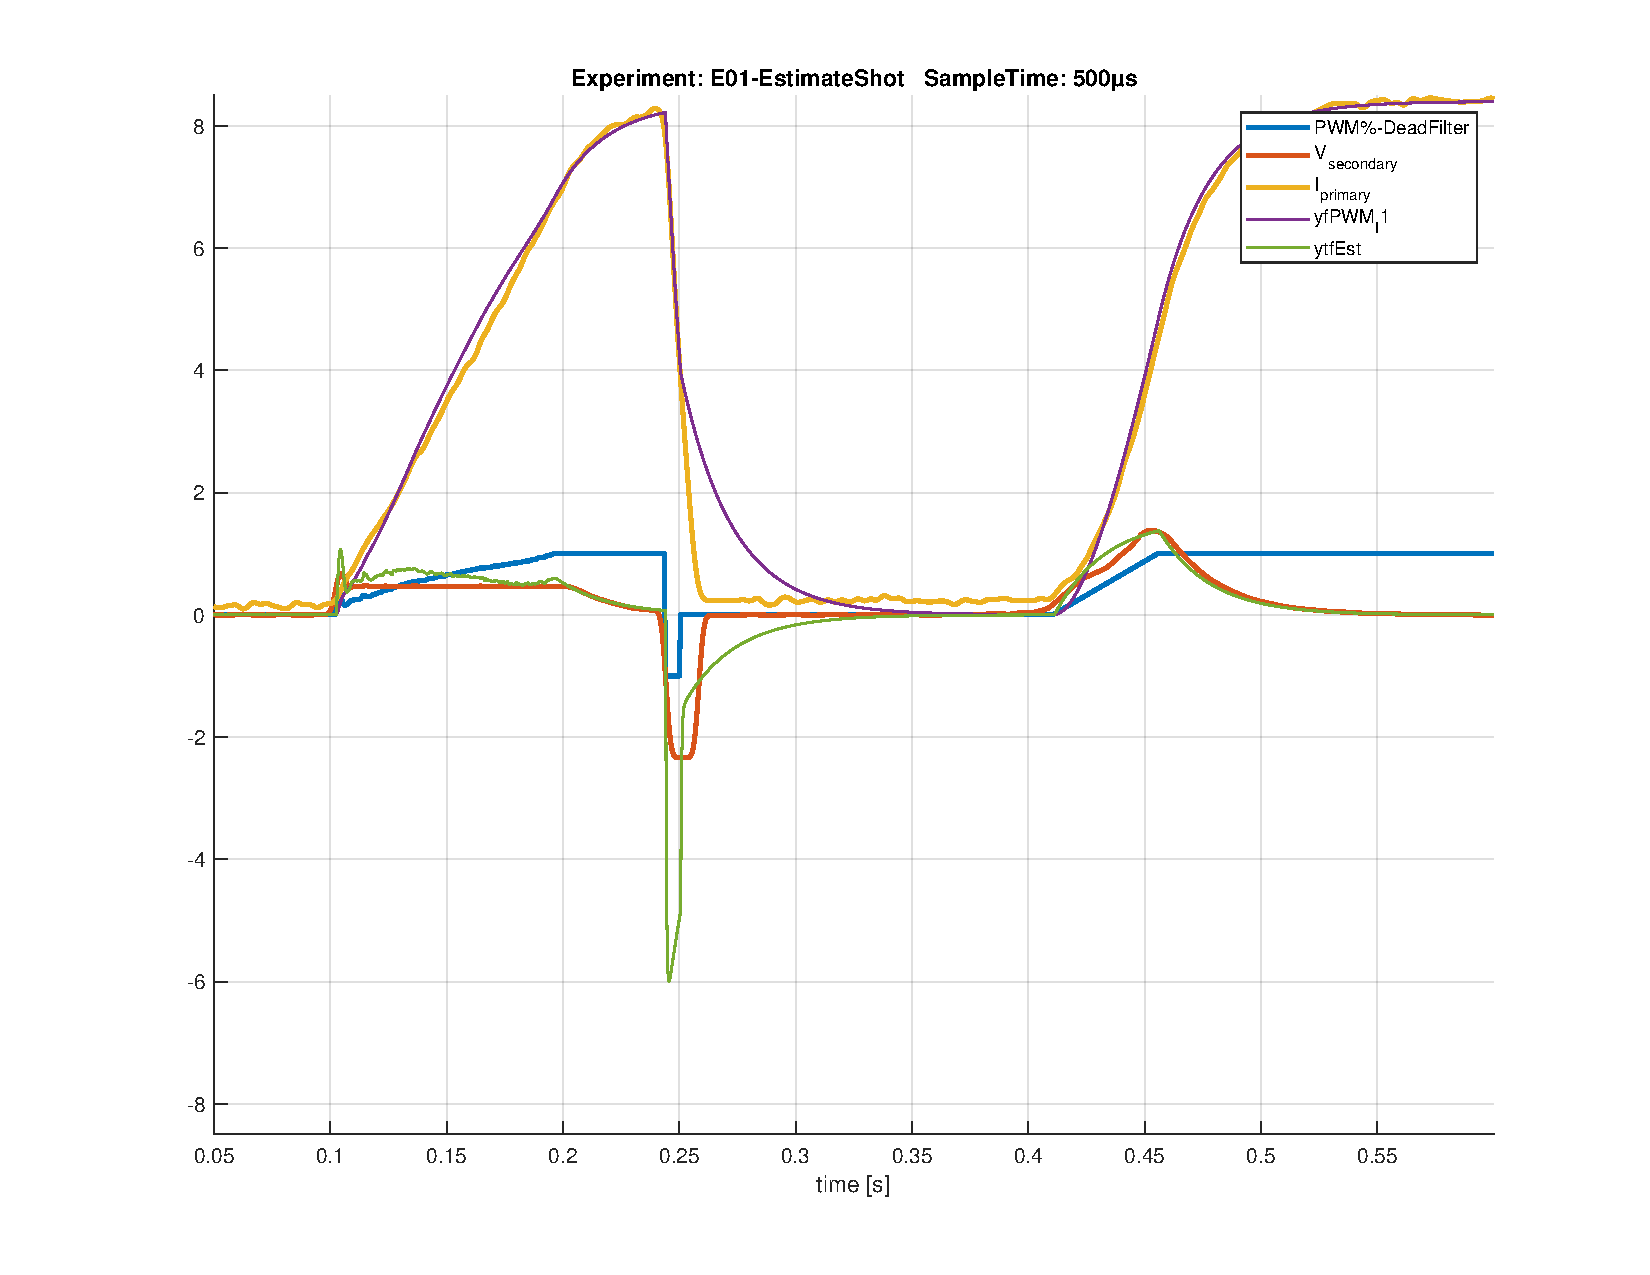
\includegraphics[width=0.9\textwidth]{Stime/E01-EstimateShot-manual-1.pdf}
\end{figure}

\begin{figure}[H]
	\centering
	\caption[Esperimento di verifica della stima 2]{Esperimento di verifica della stima 2}
	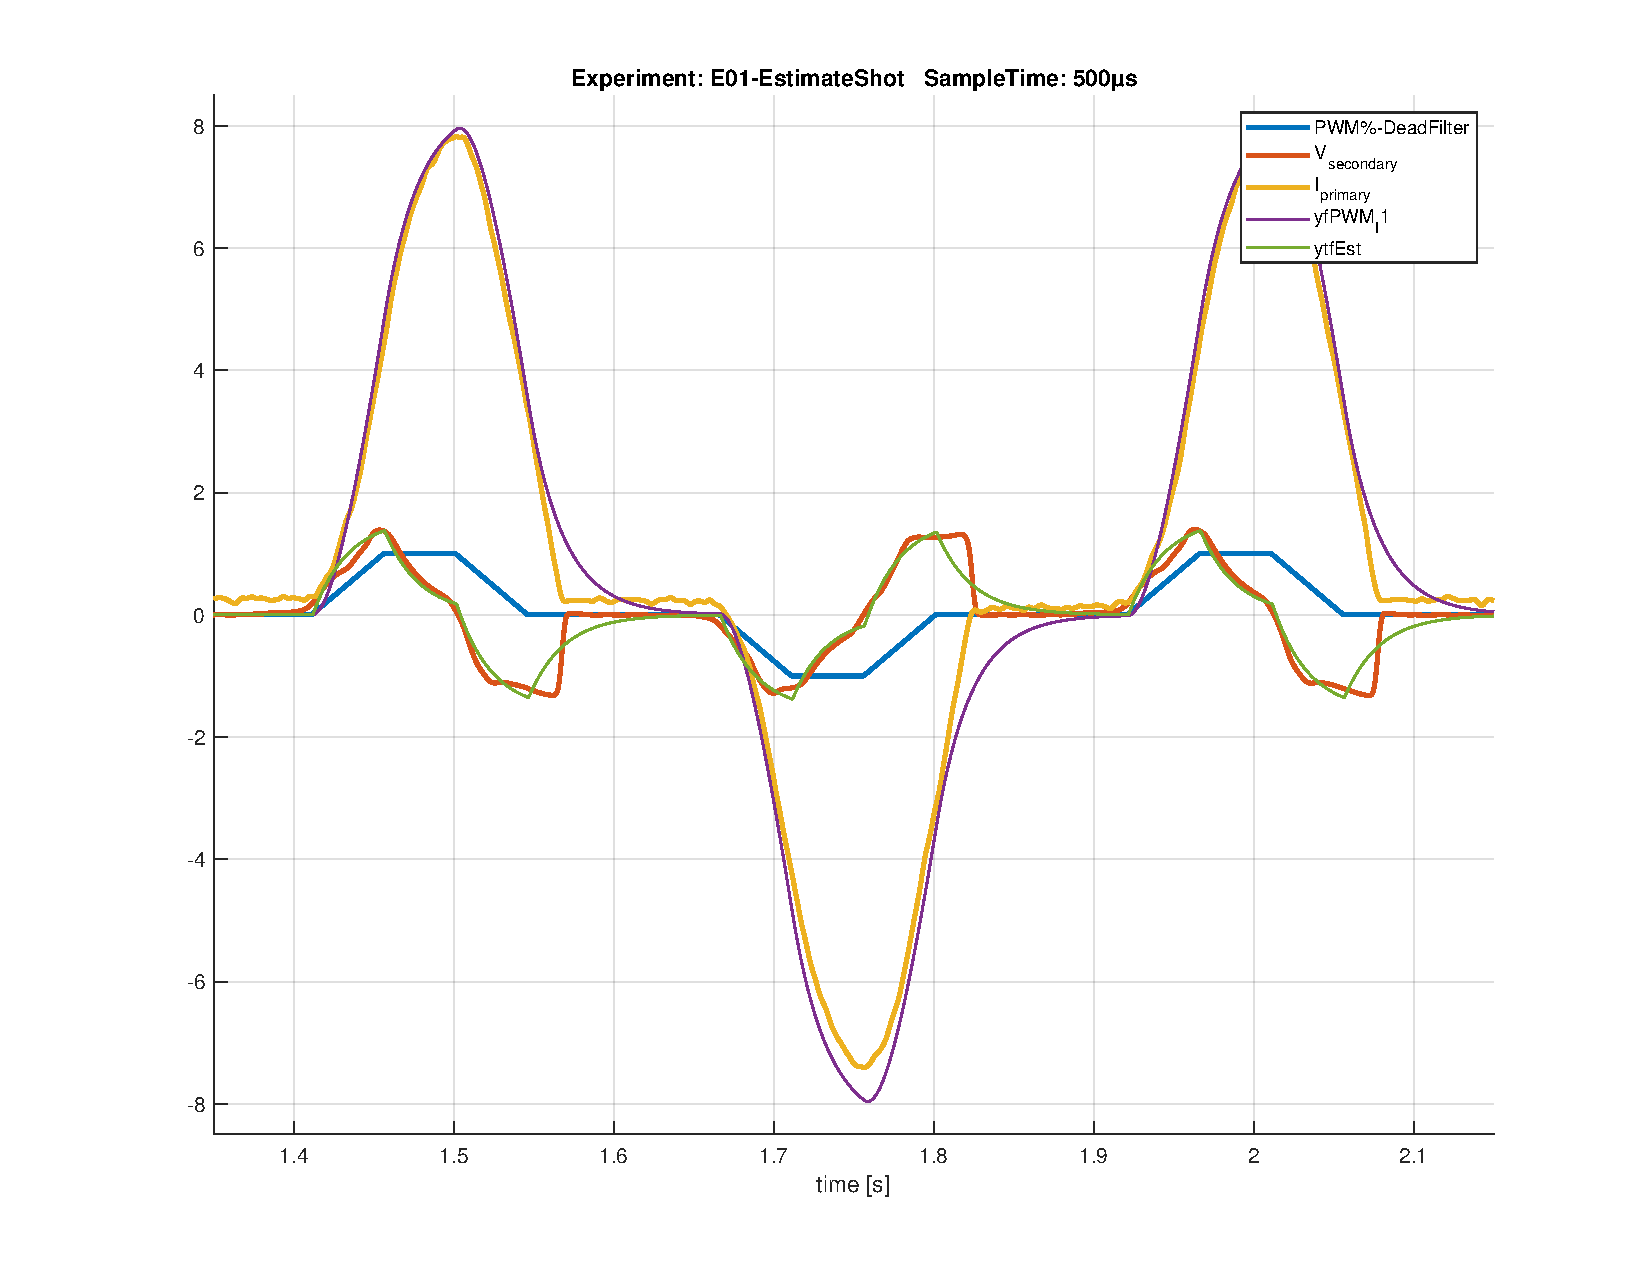
\includegraphics[width=0.9\textwidth]{Stime/E01-EstimateShot-manual-2.pdf}
\end{figure}
\vspace{-18mm}
\begin{figure}[H]
	\centering
	\caption[Esperimento di verifica della stima 3]{Esperimento di verifica della stima 3}
	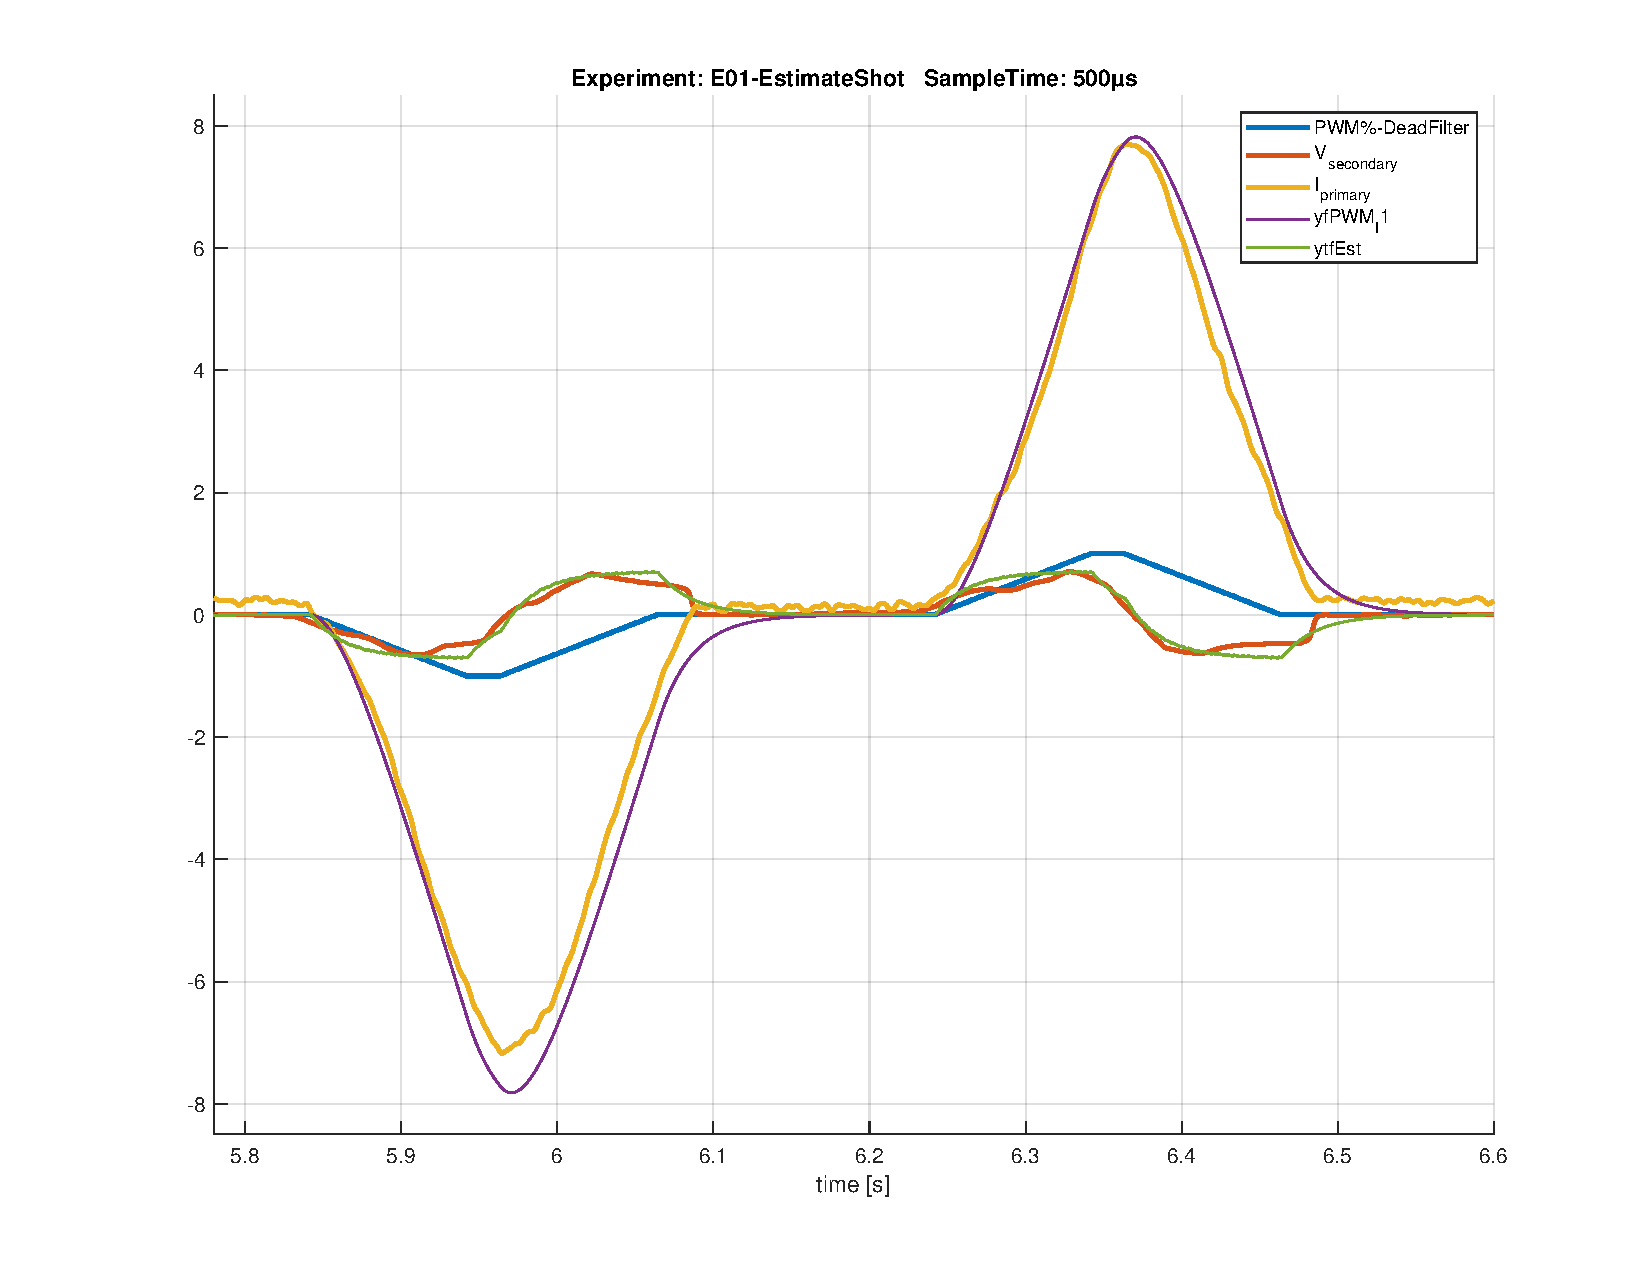
\includegraphics[width=0.9\textwidth]{Stime/E01-EstimateShot-manual-3.pdf}
\end{figure}
\noindent
Dall'analisi di questi grafici risulta chiaro che anche se il modello non è perfettamente allineato con le misure reali, a causa delle \nonLinearita del sistema originale che sono state trascurate nella creazione del modello, la dinamica simulata è rappresentativa dell'andamento reale del sistema complessivo, ed può quindi essere usata nello sviluppo teorico del controllore.\\
La funzione di trasferimento del sistema tra il segnale di PWM e arrivando alla tensione $ V_2 $ è:

\begin{Large}
	\begin{empheq}[box=\mathResult]{equation} \label{eq:StimaModelloInOut}
		\tilde{P}_{p_{wm} V_2}(s) = \frac{\num{9.1e+3}\,s}{s^2+\num{2.8e+3}\,s+\num{1.3e+5}}
	\end{empheq}
\end{Large}

\noindent
Nel seguito della tesi, questa funzione di trasferimento, con questi coefficienti, verrà usata nelle simulazioni del controllore, e ci permetterà di avere un idea qualitativa di come si comporterà il controllo una volta implementato nella realtà.\\
Come potevamo aspettarci dall'analisi teorica, i poli di $ \tilde{P}_{p_{wm} V_2} $ sono:
\begin{itemize}
	\item $ K_p \approx \num{9.1e3} $
	\item $ z_1 = 0 $ \tab\tab\tab(dalla teoria del capitolo \nameref{TrasformatoreModelloTokamak})
	\item $ s_1\approx-2752.77 $
	\item $ s_2\approx-47.2251 $
\end{itemize}
\noindent
Il ché, come ci aspettavamo dalla teoria vista nella sezione '\nameref{TrasformatoreModelloTokamak}', fa si che il sistema sia Asintoticamente Stabile poiché i poli appartengono entrambi a $ \mathbb{C}^- $, e nel caso particolare sono 2 poli semplici, il ché, anche se probabile, non era scontato.

